\newthought{\textbf{Cut Opy Mandalisa - 2020903430012 - TRKJ 3B}}

\newday{\textbf{1-2 Desember 2022- Instalasi dan Konfigurasi Hadoop}}
\begin{enumerate}
\item Kendala dan Solusi\\
% jelaskan kendala dan penyebab yang dialami saat mengikuti praktikum serta solusi atau langkah-langkah yang telah dilakukan
Pada Praktikum pertama yaitu penginstalan apache hadoop.kendala yang didapat tidak bisa membuka firefox kemudian solusinya dengan menginstal firefox baru.

\begin{figure}[!ht]
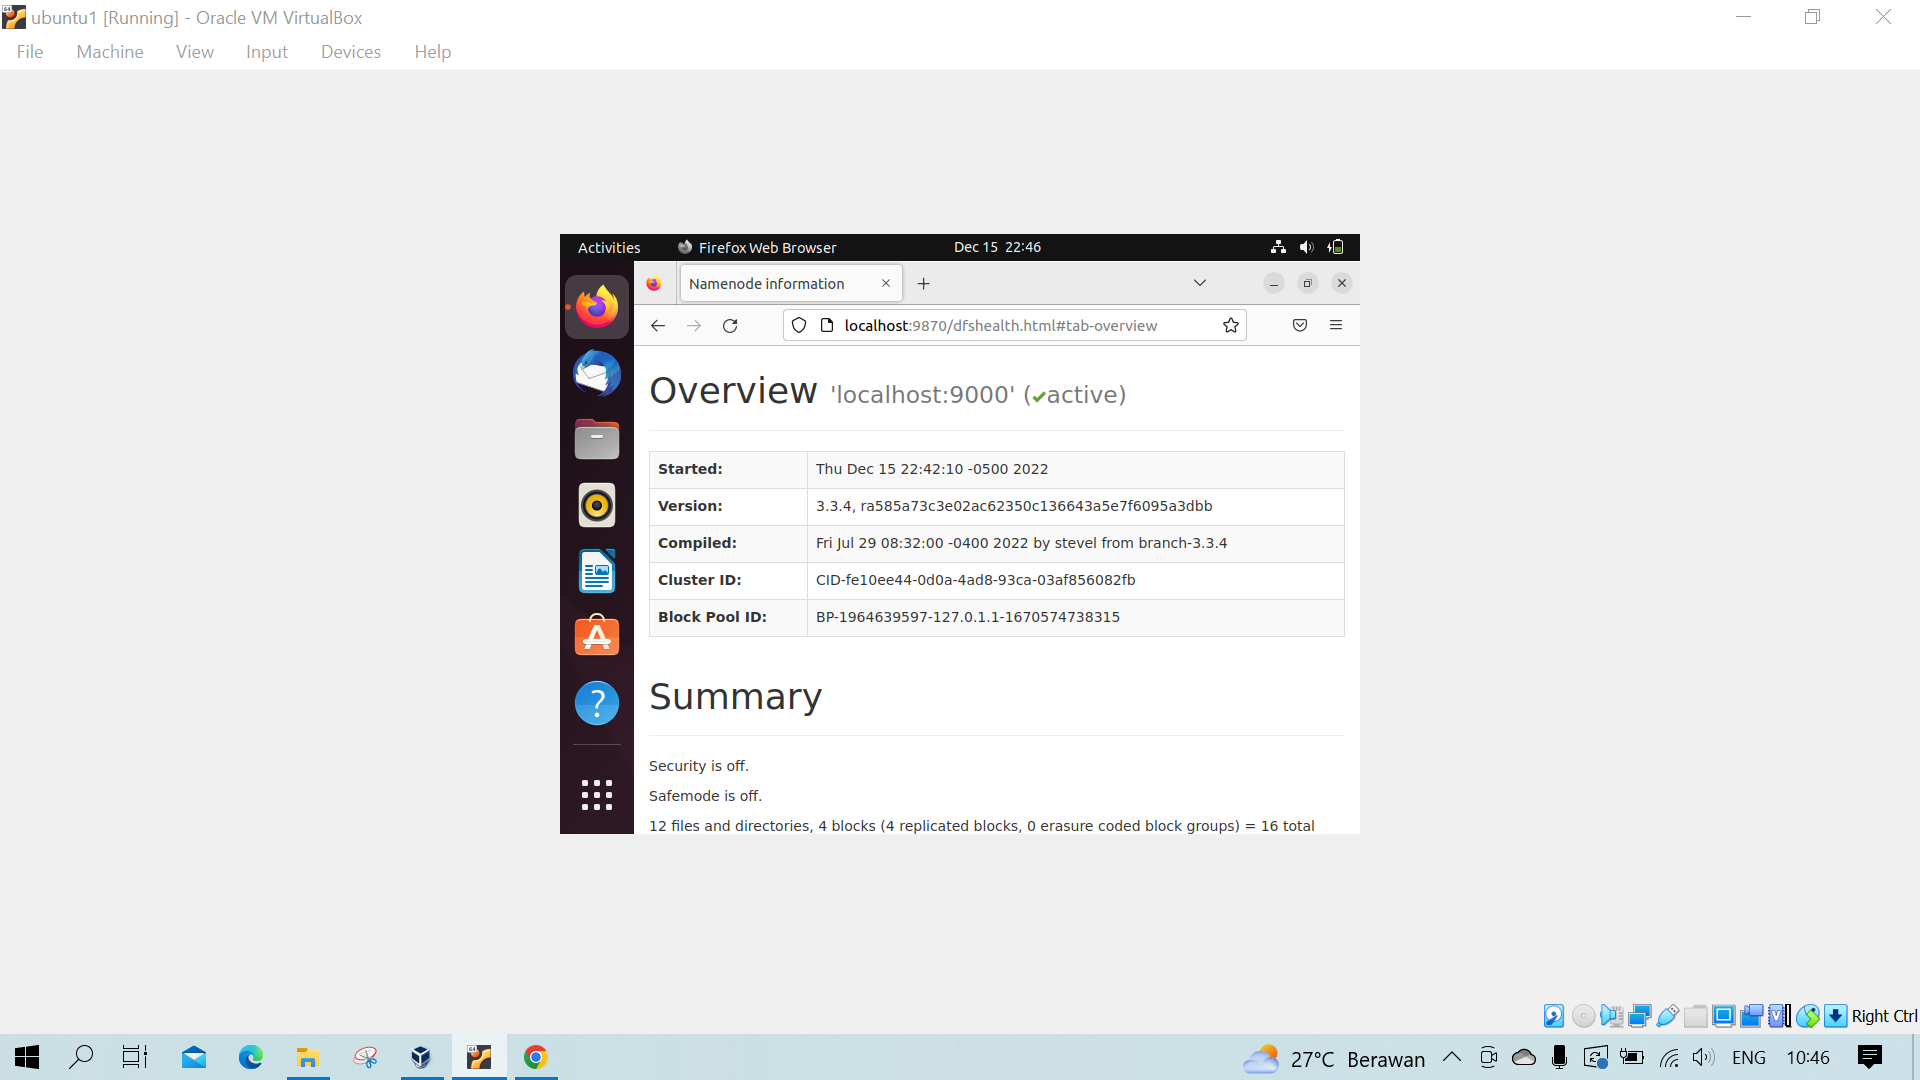
\includegraphics[width=\textwidth]{CutOpyMandalisa/01}
\caption{hasil dari cek hadoop service}
\label{gam:perkuliahan-25-11}
\end{figure}

\begin{figure}[!ht]
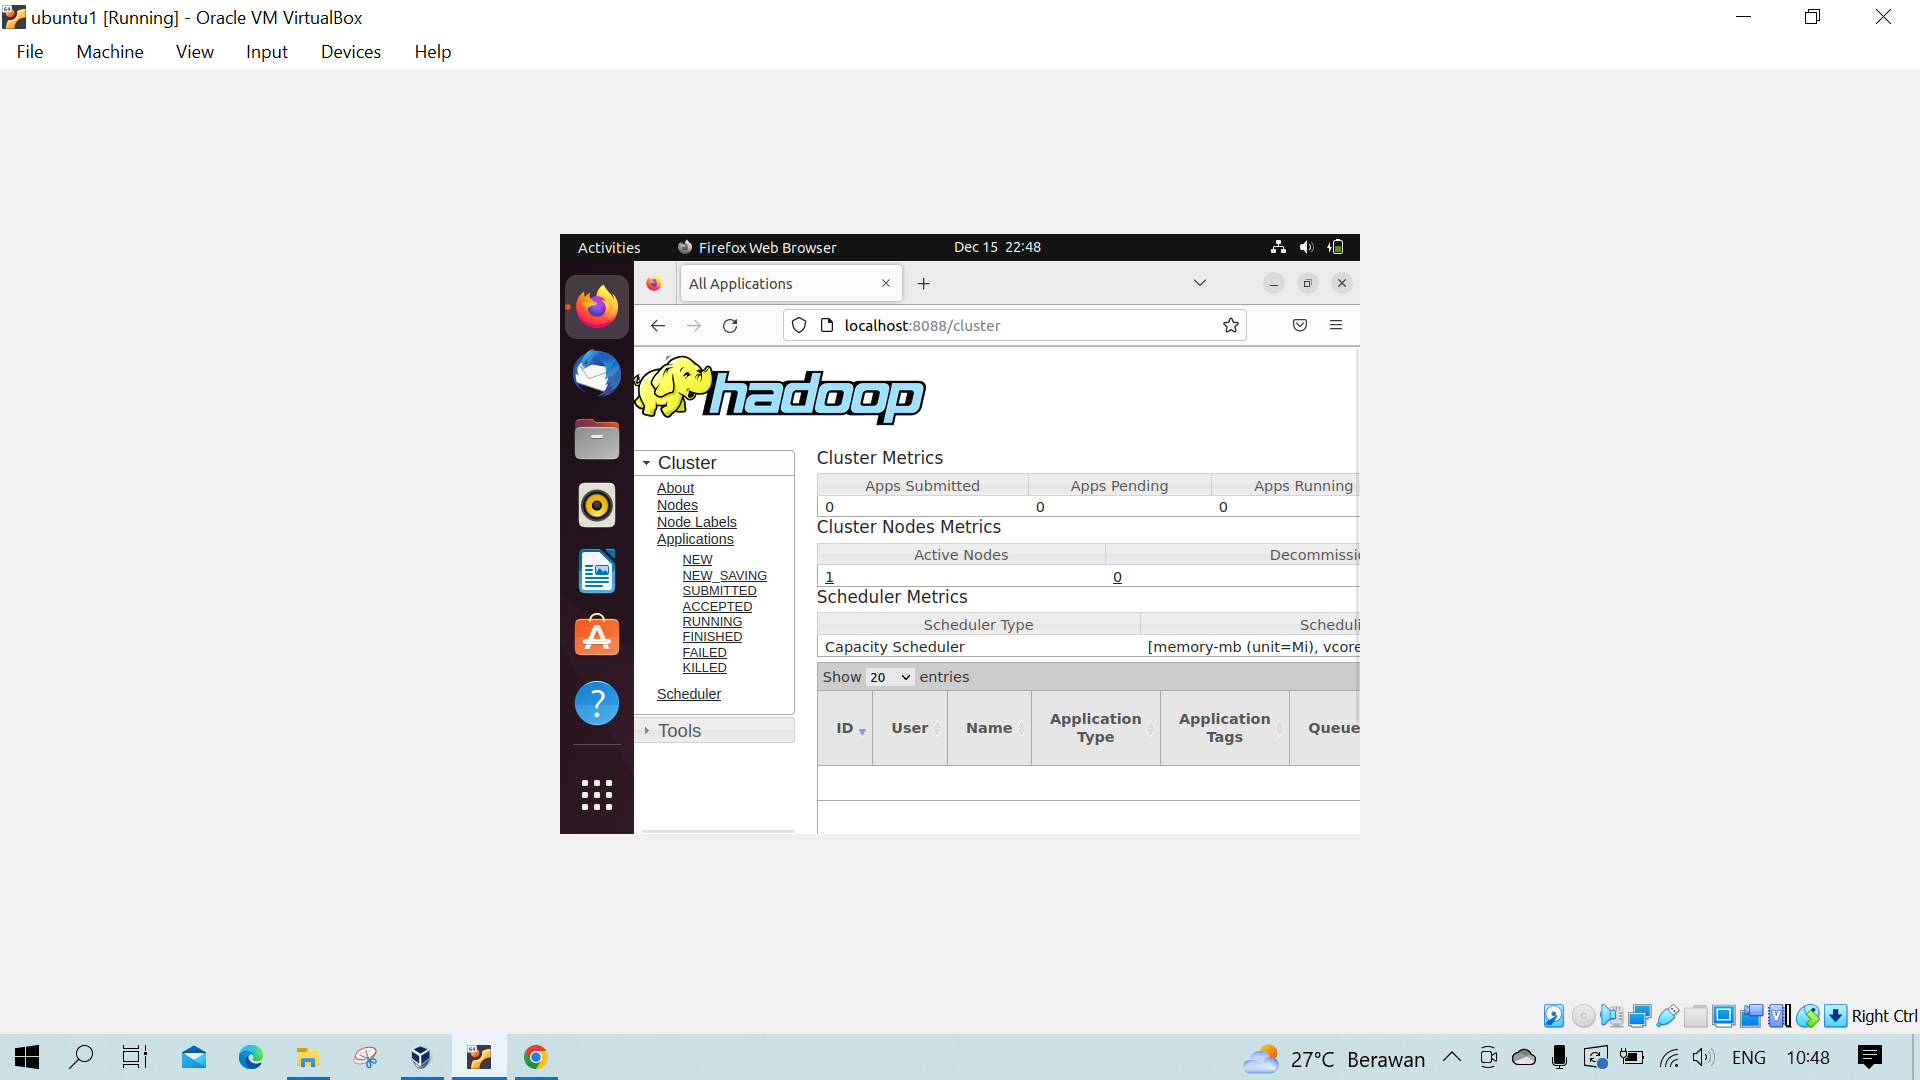
\includegraphics[width=\textwidth]{CutOpyMandalisa/02}
\caption{hasil cek hadoop service}
\label{gam:perkuliahan-25-11}
\end{figure}

\item Kesimpulan\\
% berikan kesimpulan dari praktikum yang telah dikerjkan
Behasil mendownload dan menginstal Apache hadoop dan sudah bisa dijalankan
\end{enumerate}


\newday{\textbf{08 Desember 2022-WordCount bawaan Hadoop}}
\begin{enumerate}

\item Kendala dan Solusi
\newpage
% jelaskan kendala dan penyebab yang dialami saat mengikuti praktikum serta solusi atau langkah-langkah yang telah dilakukan
Pada praktikum ini membuat program WordCount bawaan Hadoop. Pada melakukan praktikum tidak ada kendala hanya erorr dikarenakan salah memasukkan perintah.

\begin{figure}[!ht]
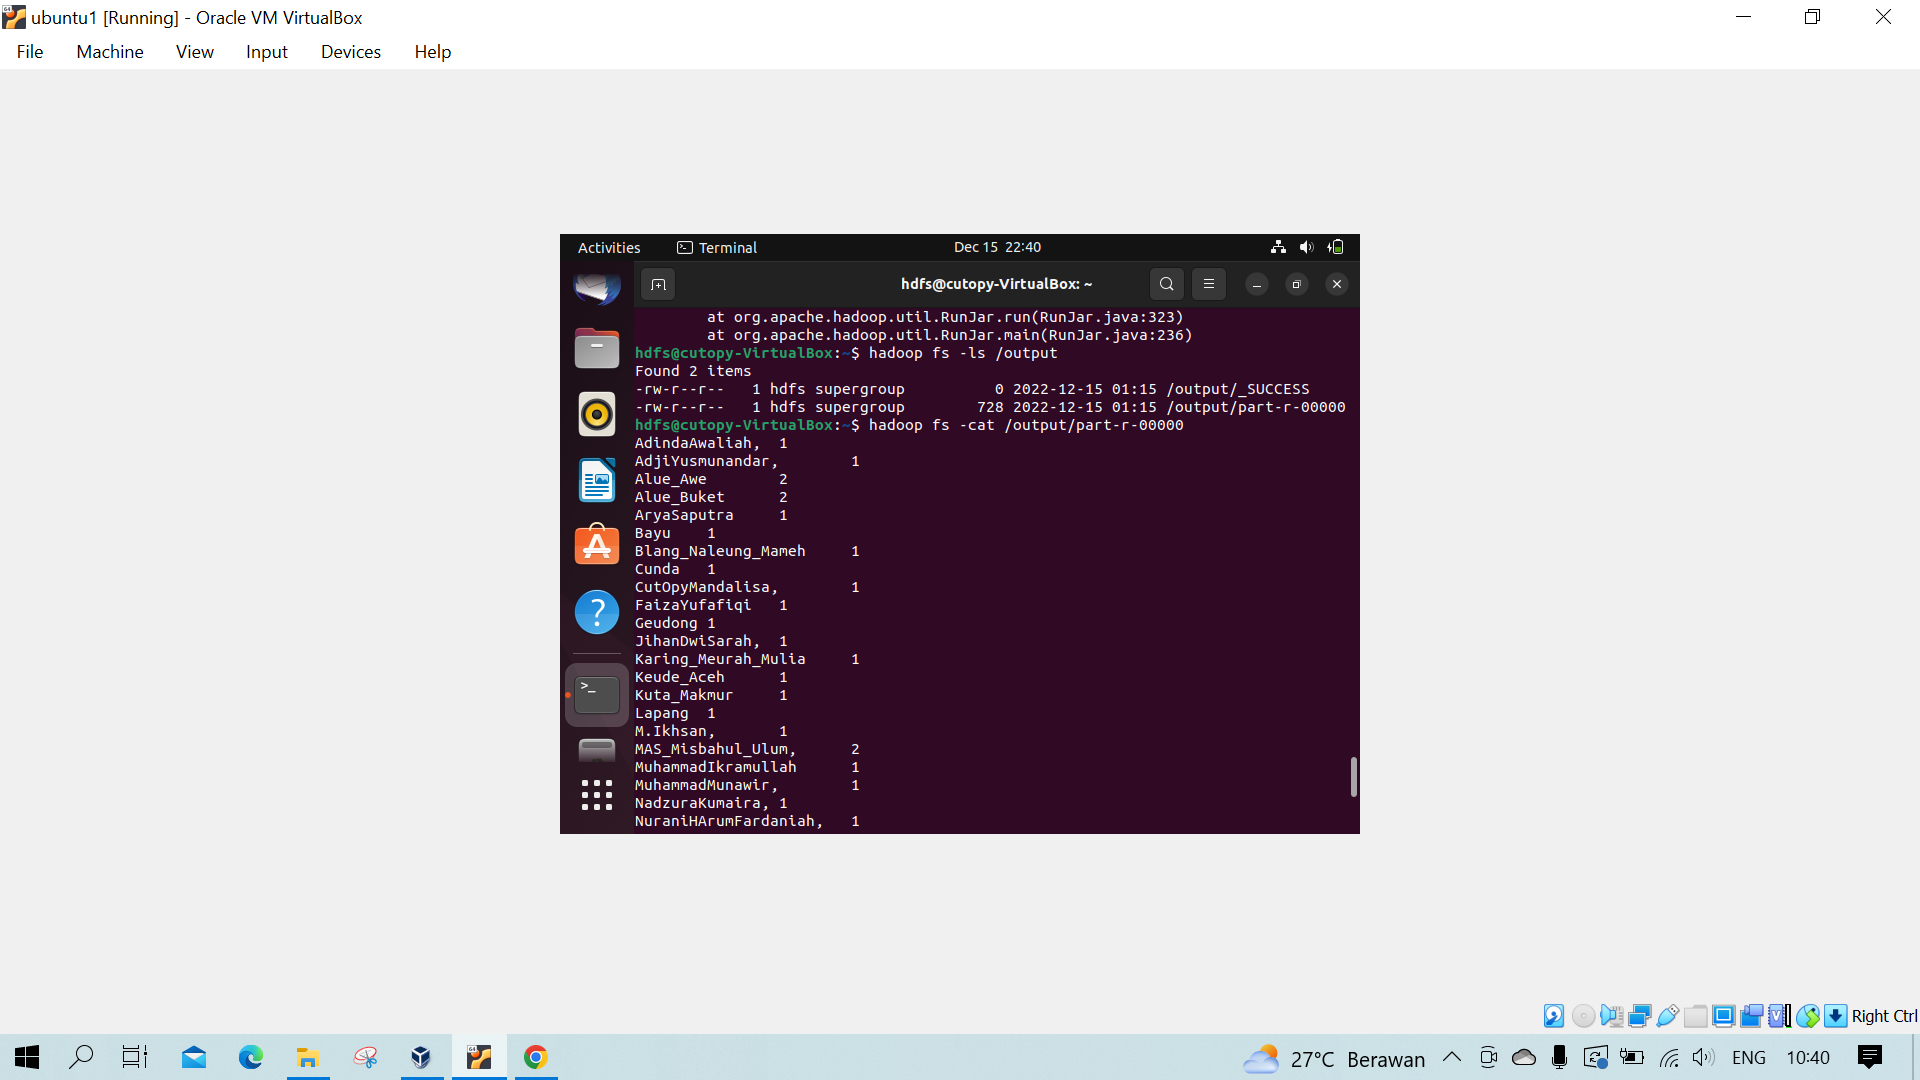
\includegraphics[width=\textwidth]{CutOpyMandalisa/03}
\caption{hasil WordCount bawaan Hadoop}
\label{gam:perkuliahan-25-11}
\end{figure}

\item Kesimpulan\\
% berikan kesimpulan dari praktikum yang telah dikerjkan
Pada praktikum ini untuk memahami proses cara kerja pada hadoop dalam memproses data input sehingga menghasilkan output.Wordcount merupakan program untuk menghitung jumlah kata dalam input.
\end{enumerate}


\newday{\textbf{09 Desember 2022-WordCount dengan Java}}
\begin{enumerate}
\item Kendala dan Solusi\\
% jelaskan kendala dan penyebab yang dialami saat mengikuti praktikum serta solusi atau langkah-langkah yang telah dilakukan
Pada praktikum ini membuat program WordCount dengan java.Pada saat melakukan praktikum terdapat error akan tetapi erorrnya disebabkan salah memasukkan perintah codingannya.solusinya harus lebih teliti saat memasukkan codingan tersebut.

\begin{figure}[!ht]
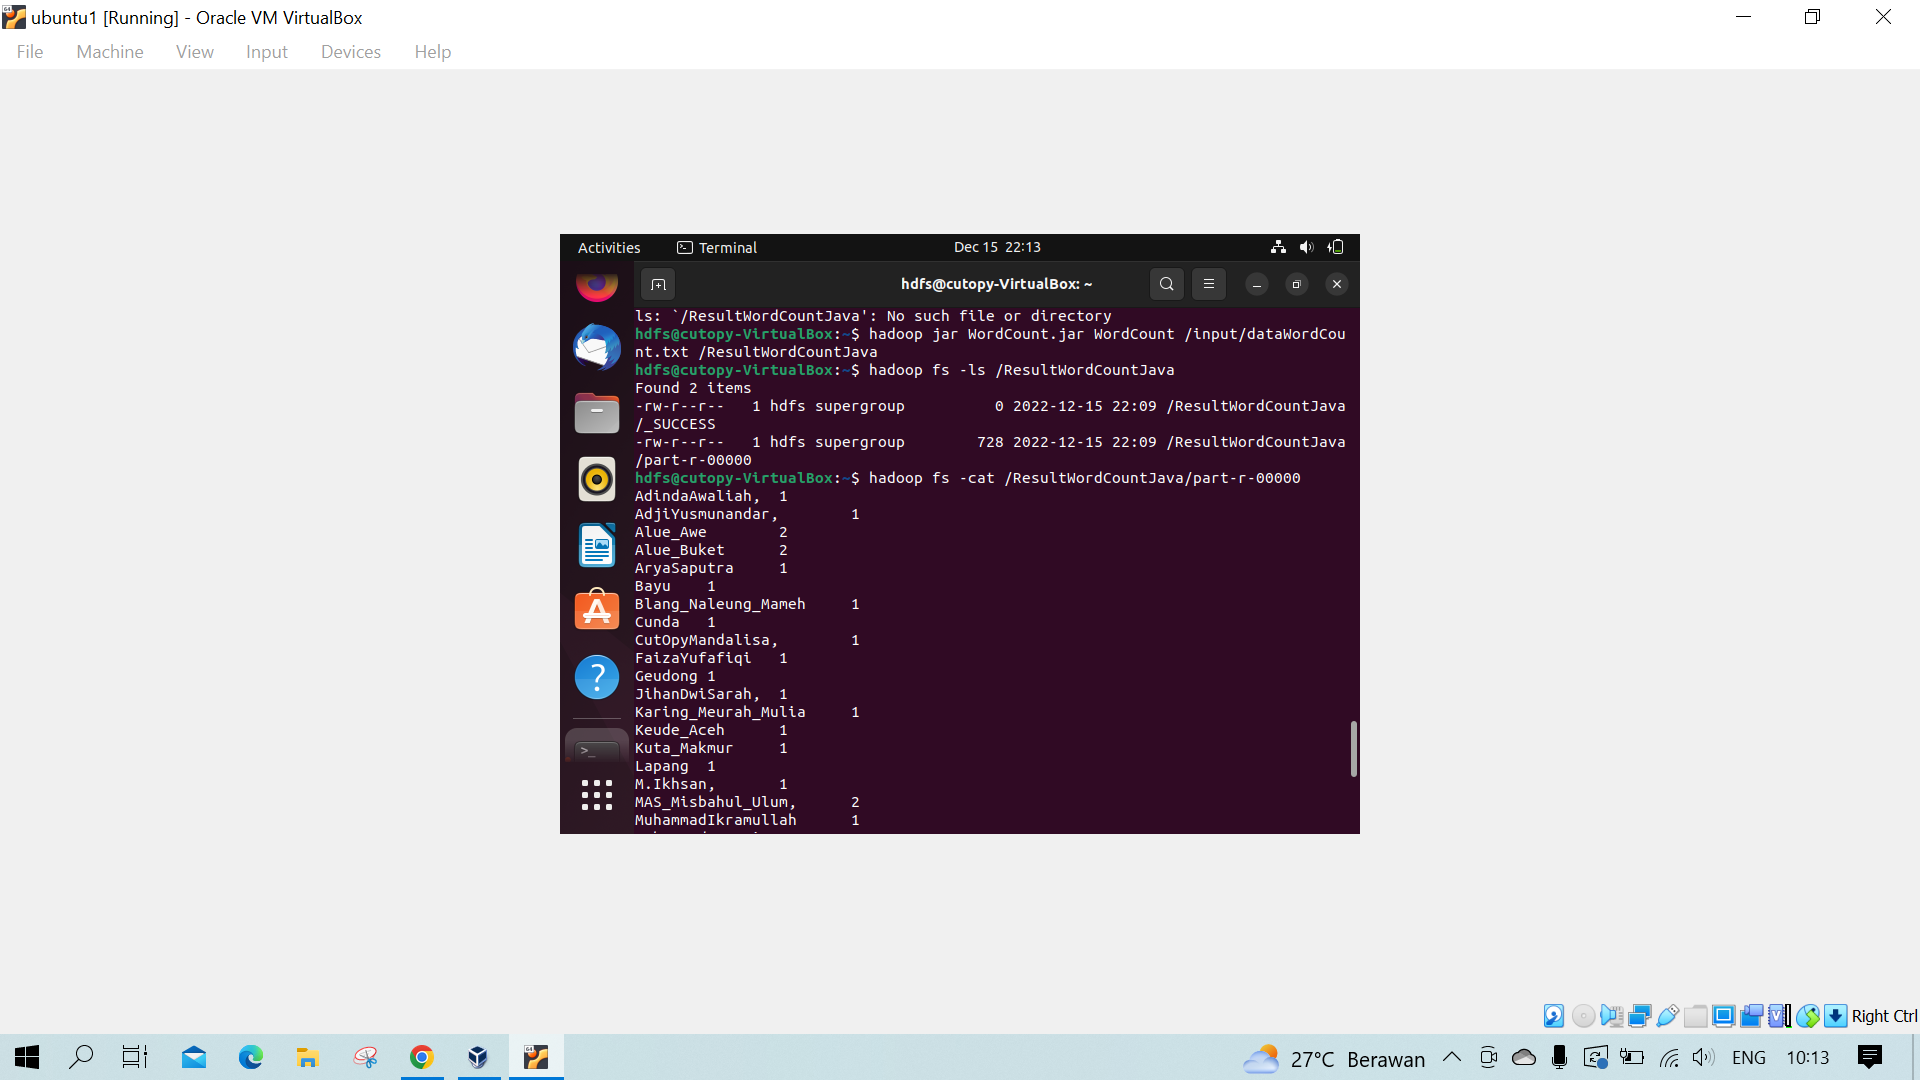
\includegraphics[width=\textwidth]{CutOpyMandalisa/04}
\caption{hasil wordCount dengan java}
\label{gam:perkuliahan-25-11}
\end{figure}

\item Kesimpulan\\
% berikan kesimpulan dari praktikum yang telah dikerjkan
Berhasil menjalankan program WordCount dengan java.
\end{enumerate}


\newday{\textbf{15 Desember 2022}}
\begin{enumerate}
\item Kendala dan Solusi
% jelaskan kendala dan penyebab yang dialami saat mengikuti praktikum serta solusi atau langkah-langkah yang telah dilakukan

\item Kesimpulan
% berikan kesimpulan dari praktikum yang telah dikerjkan
\end{enumerate}


\newday{\textbf{16 Desember 2022}}
\begin{enumerate}
\item Kendala dan Solusi
% jelaskan kendala dan penyebab yang dialami saat mengikuti praktikum serta solusi atau langkah-langkah yang telah dilakukan

\item Kesimpulan
% berikan kesimpulan dari praktikum yang telah dikerjkan
\end{enumerate}